
	Si bien hasta ahora en la simulación se han utilizado datos de las mediciones en forma equiespaciada, en las aplicaciones prácticas muchas veces no se sabe en qué momento se recibirá la próxima medición, o incluso puede darse que recibamos información de distintos sensores con distinta frecuencia. El objetivo de este punto es ver cómo se comporta el filtro de Kalman ante la falta o pérdida de datos en algunos instantes. Para poder simular esto disponemos de dos mecanismos distintos: el primer método para simularlo es utilizando una matriz de salida $C_d$ dinámica que se modifique en función de los datos de los sensores disponibles en un determinado instante. La segunda variante es utilizar una matriz $C_d$ de tamaño fijo, e insertar ceros en lugar de las matrices de identidad por cada vez que se pierde un dato o no se dispone de una medición de ese sensor. Dado que disponer de memoria dinámica para la matriz $C_d$ es un poco mas costoso en los sistemas reales, se ha optado por la segunda alternativa.
	
	En la figura \ref{fig:ej7_1} puede verse lo que sucede si se pierden un 10 \% de las mediciones. En este caso el error de estimación no es severo. Por otro lado en la figura \ref{fig:ej7_2} se observa lo que sucede cuando se pierden un 90 \% de las mediciones. Si el filtro deja de recibir información de los sensores continuará estimando con la dinámica del sistema. En el segundo caso se observa que cada vez que ocurren largos lapsos en los que no recibe mediciones el error de estimación crece cada vez más, hasta que se recibe una nueva medición que lo vuelve a colocar en la trayectoria.
	
	\begin{figure}[H]
		\centering
		%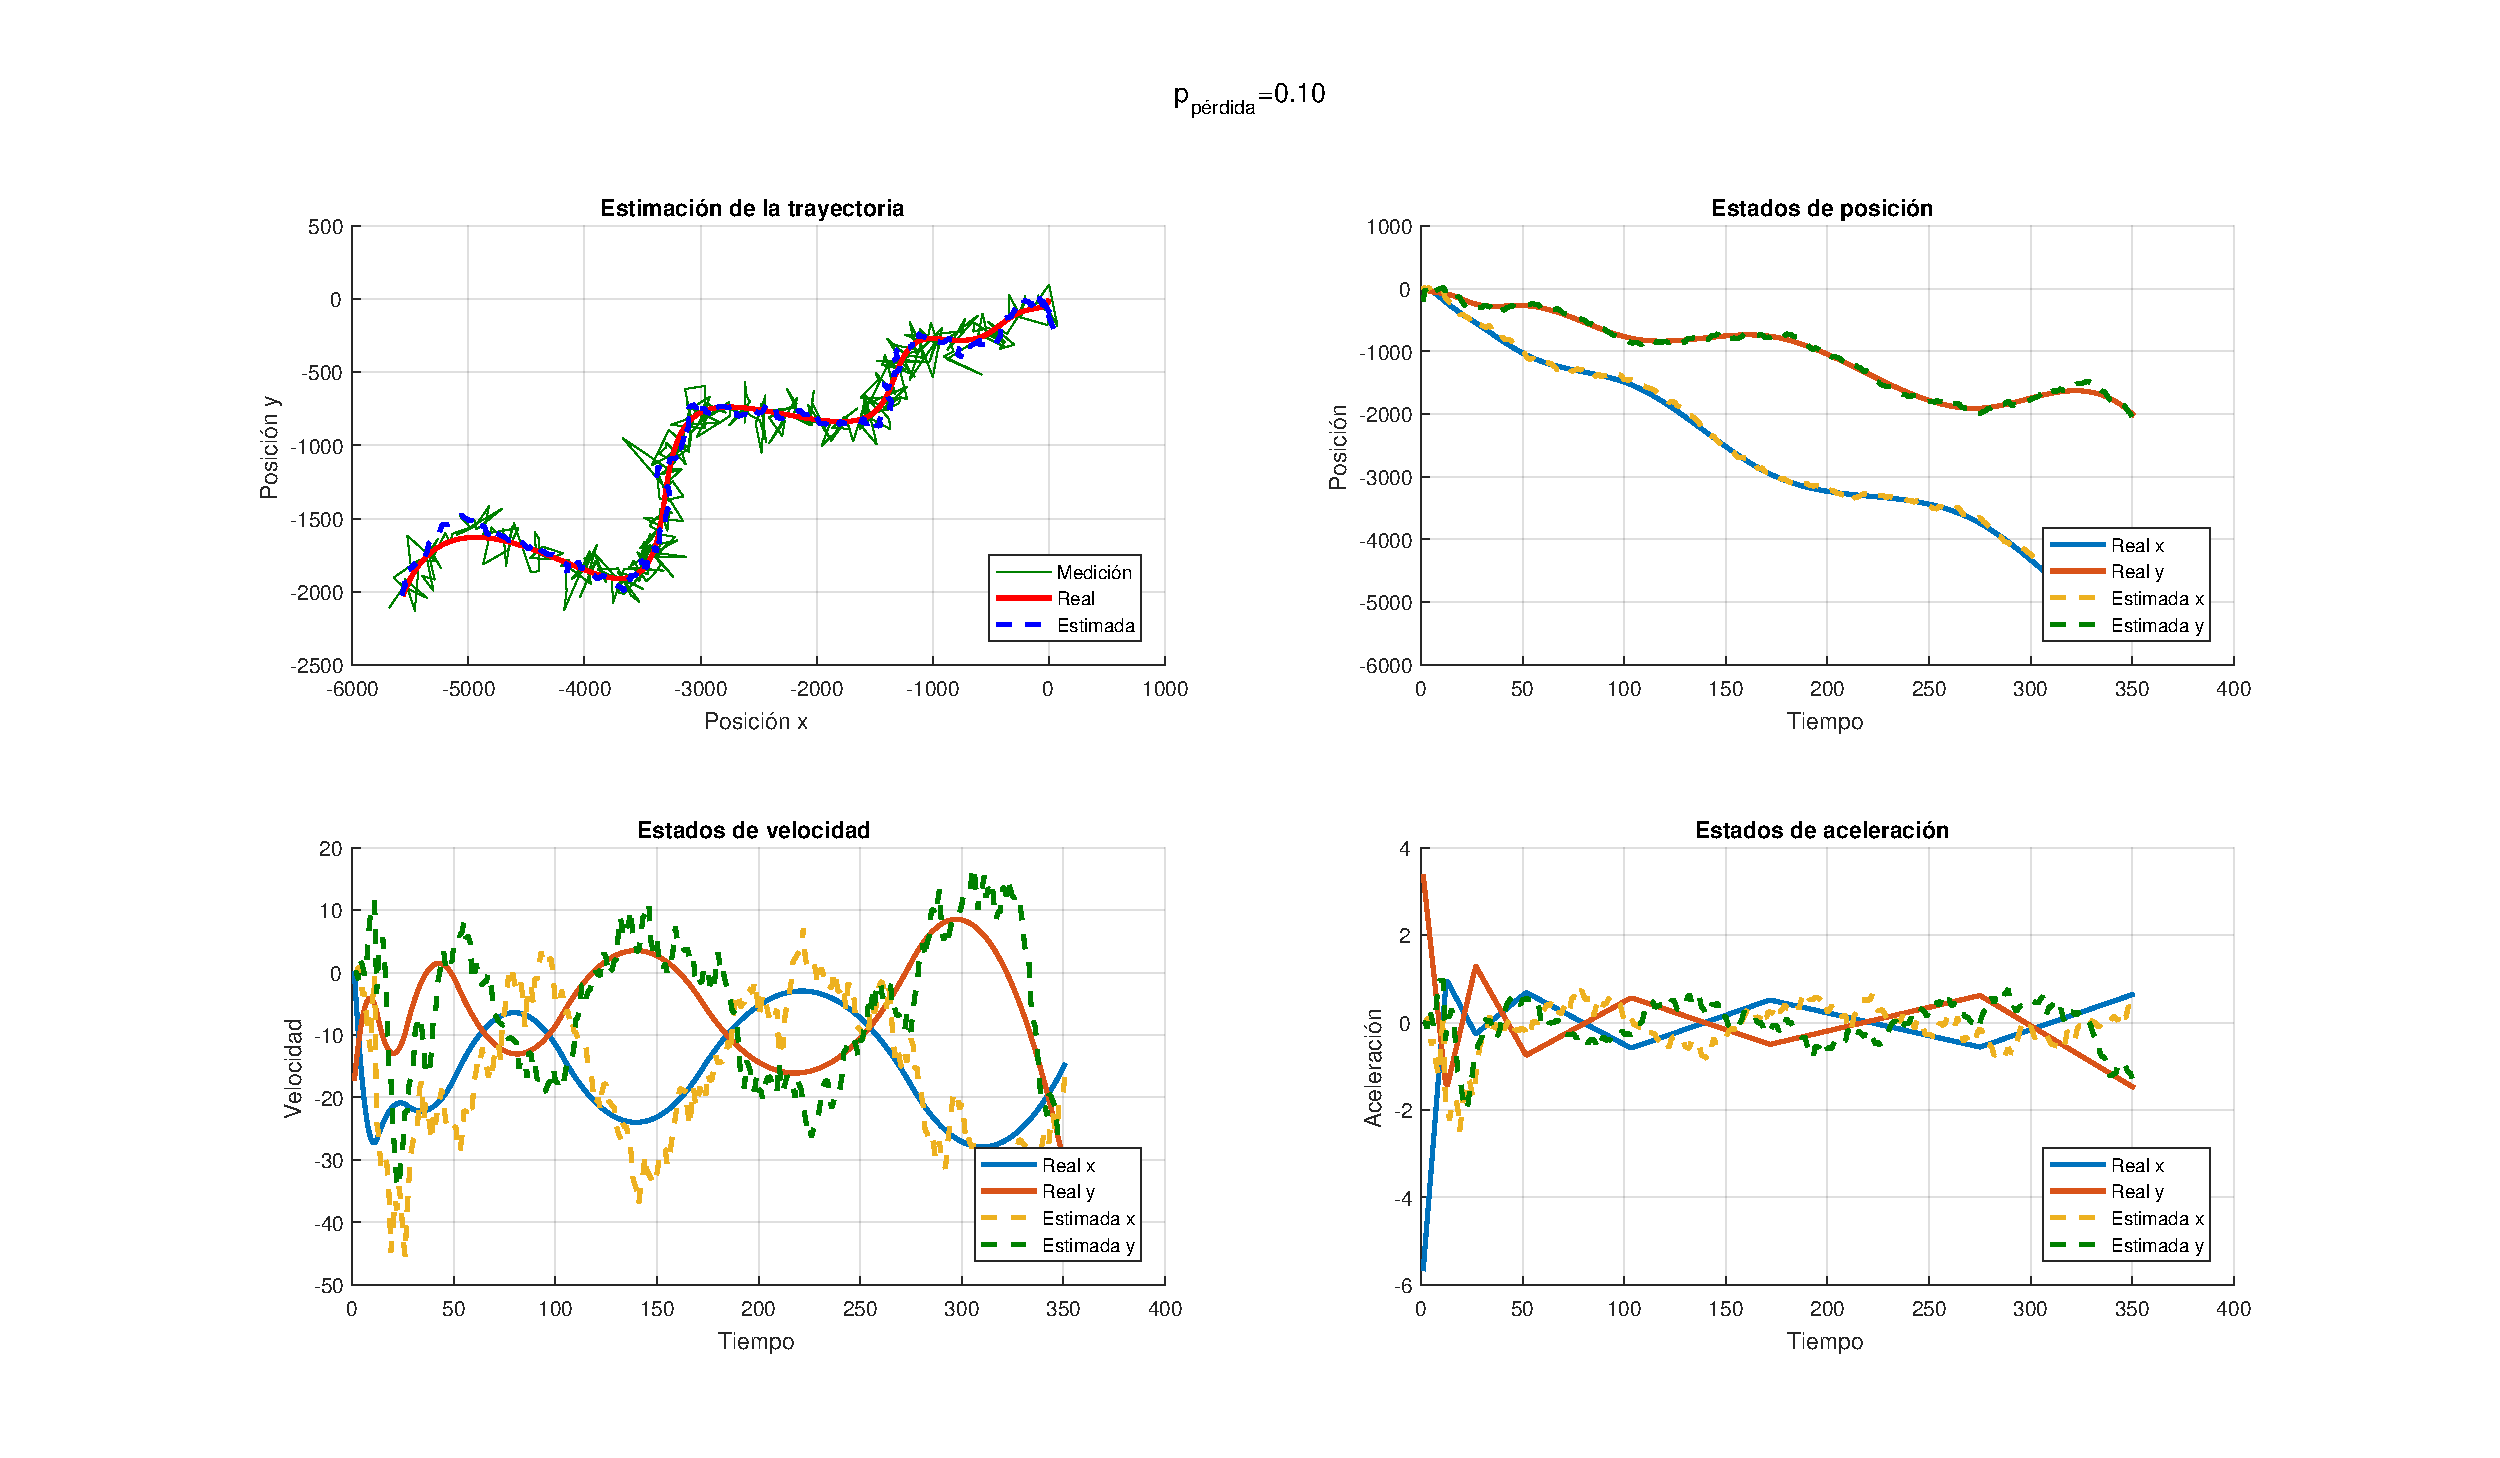
\includegraphics[width=1.0\textwidth,keepaspectratio]{Figuras/graf_ej7_1.pdf}
		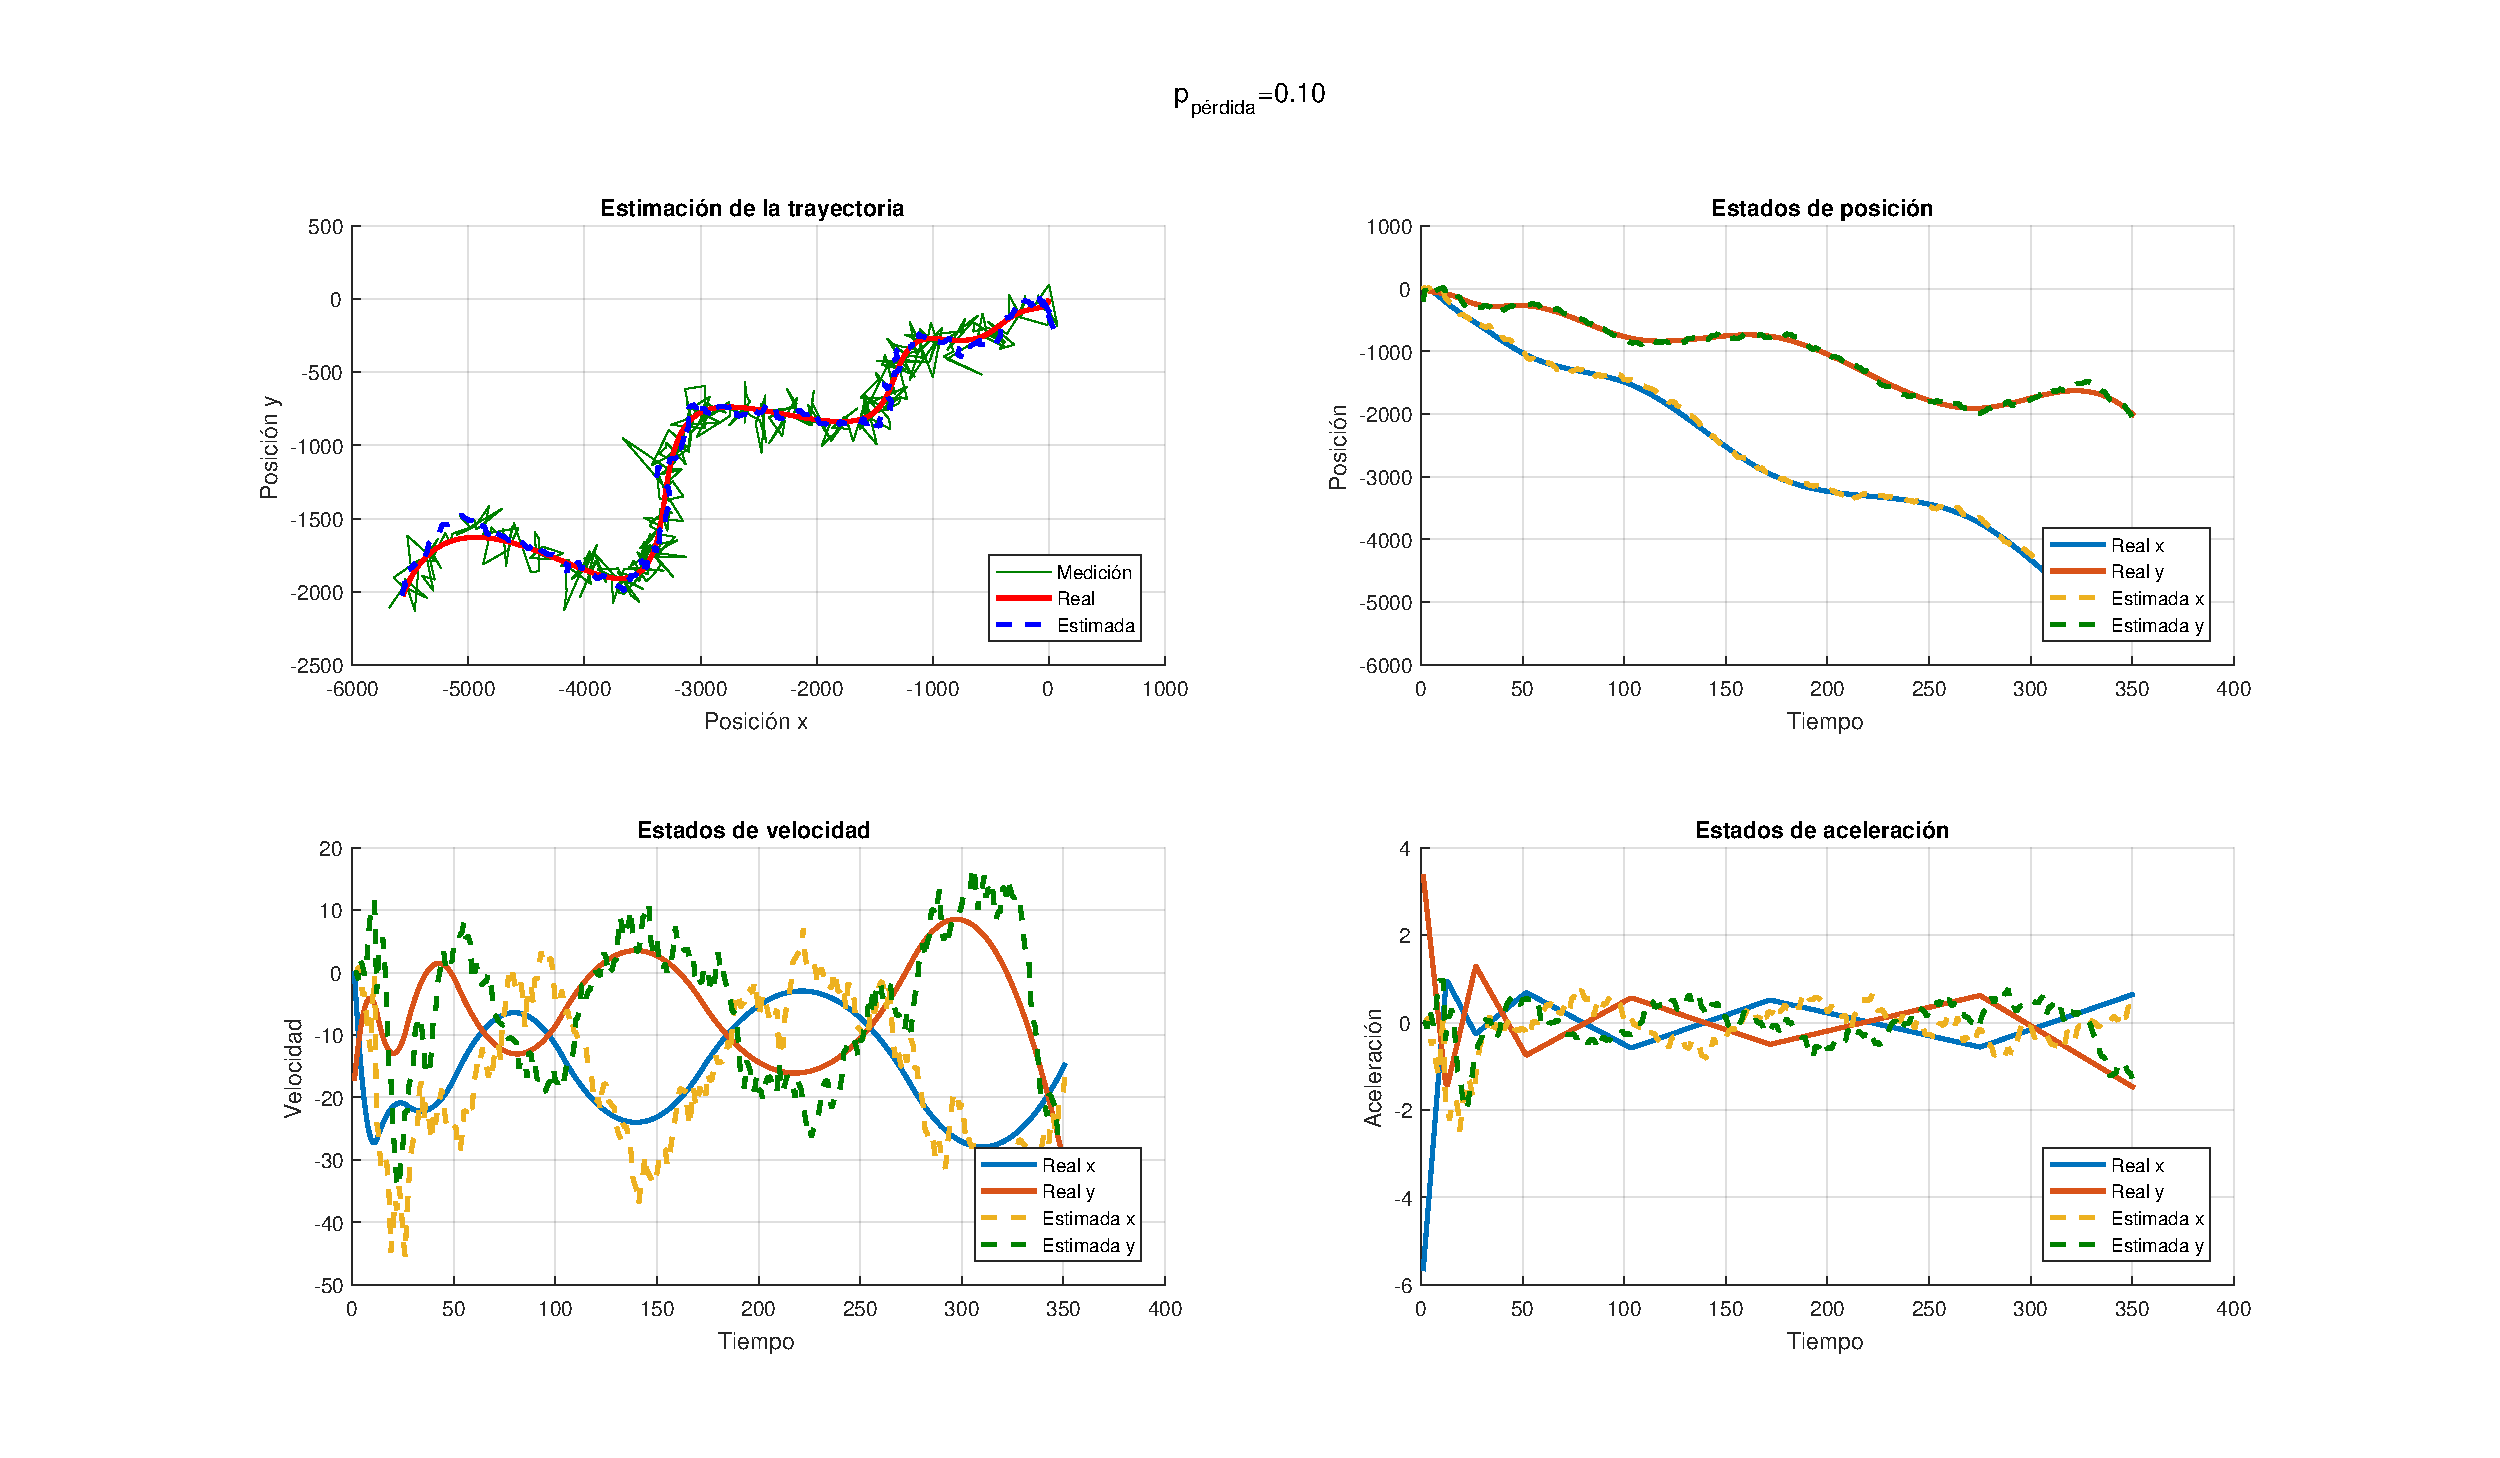
\includegraphics[scale=0.5,trim={6,5cm 0 0 0}]{Figuras/graf_ej7_1.pdf}
		\caption{Estimación De Trayectoria - Perdida Del 10 \%}
		\label{fig:ej7_1}
	\end{figure}
	
	\begin{figure}[H]
		\centering
		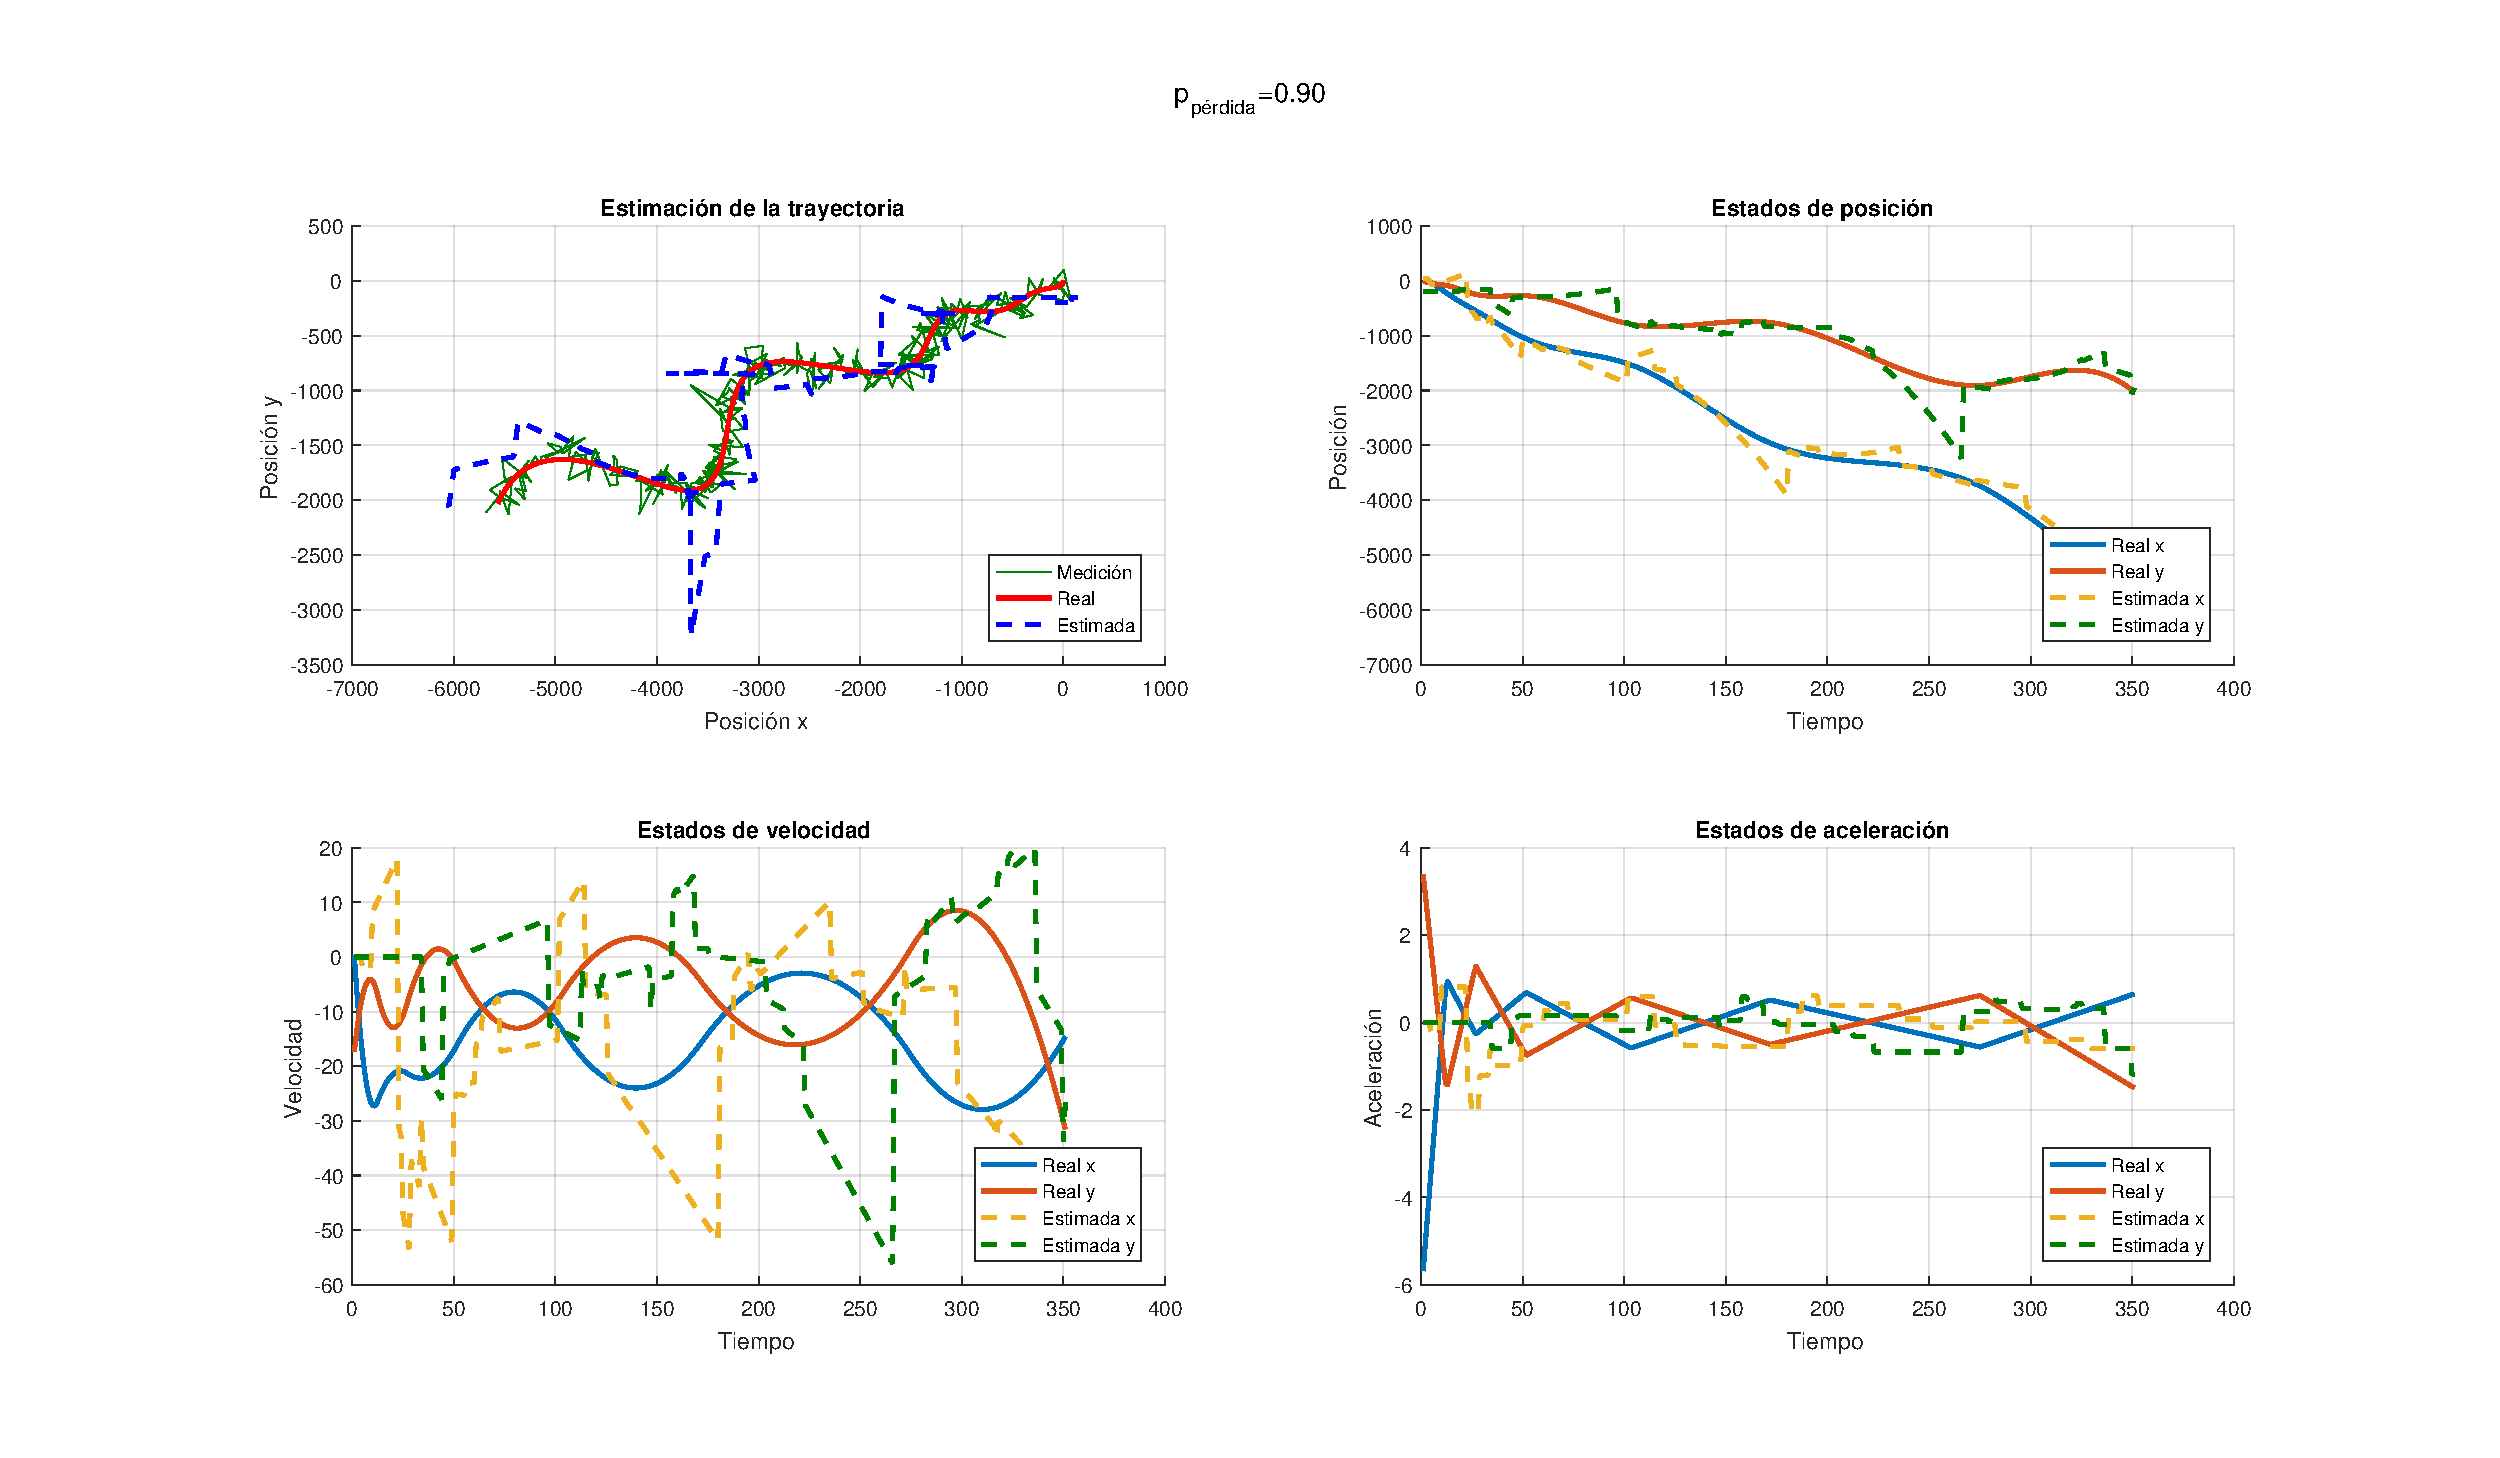
\includegraphics[scale=0.5,trim={6,5cm 0 0 0}]{Figuras/graf_ej7_2.pdf}
		\caption{Estimación De Trayectoria - Perdida Del 90 \%}
		\label{fig:ej7_2}
	\end{figure}
	
	En las figuras \ref{fig:ej7_1_inov} y \ref{fig:ej7_1_inov} podemos ver la autocorrelación de las innovaciones. Cuanto más se parezcan a ruido blanco, mejor es la estimación. Es decir, todo lo que no puede predecir el filtro corresponde a ruido blanco. También resulta notable que cuantas menos mediciones se tiene, menos se da esta propiedad.
	
	\begin{figure}[H]
		\centering
		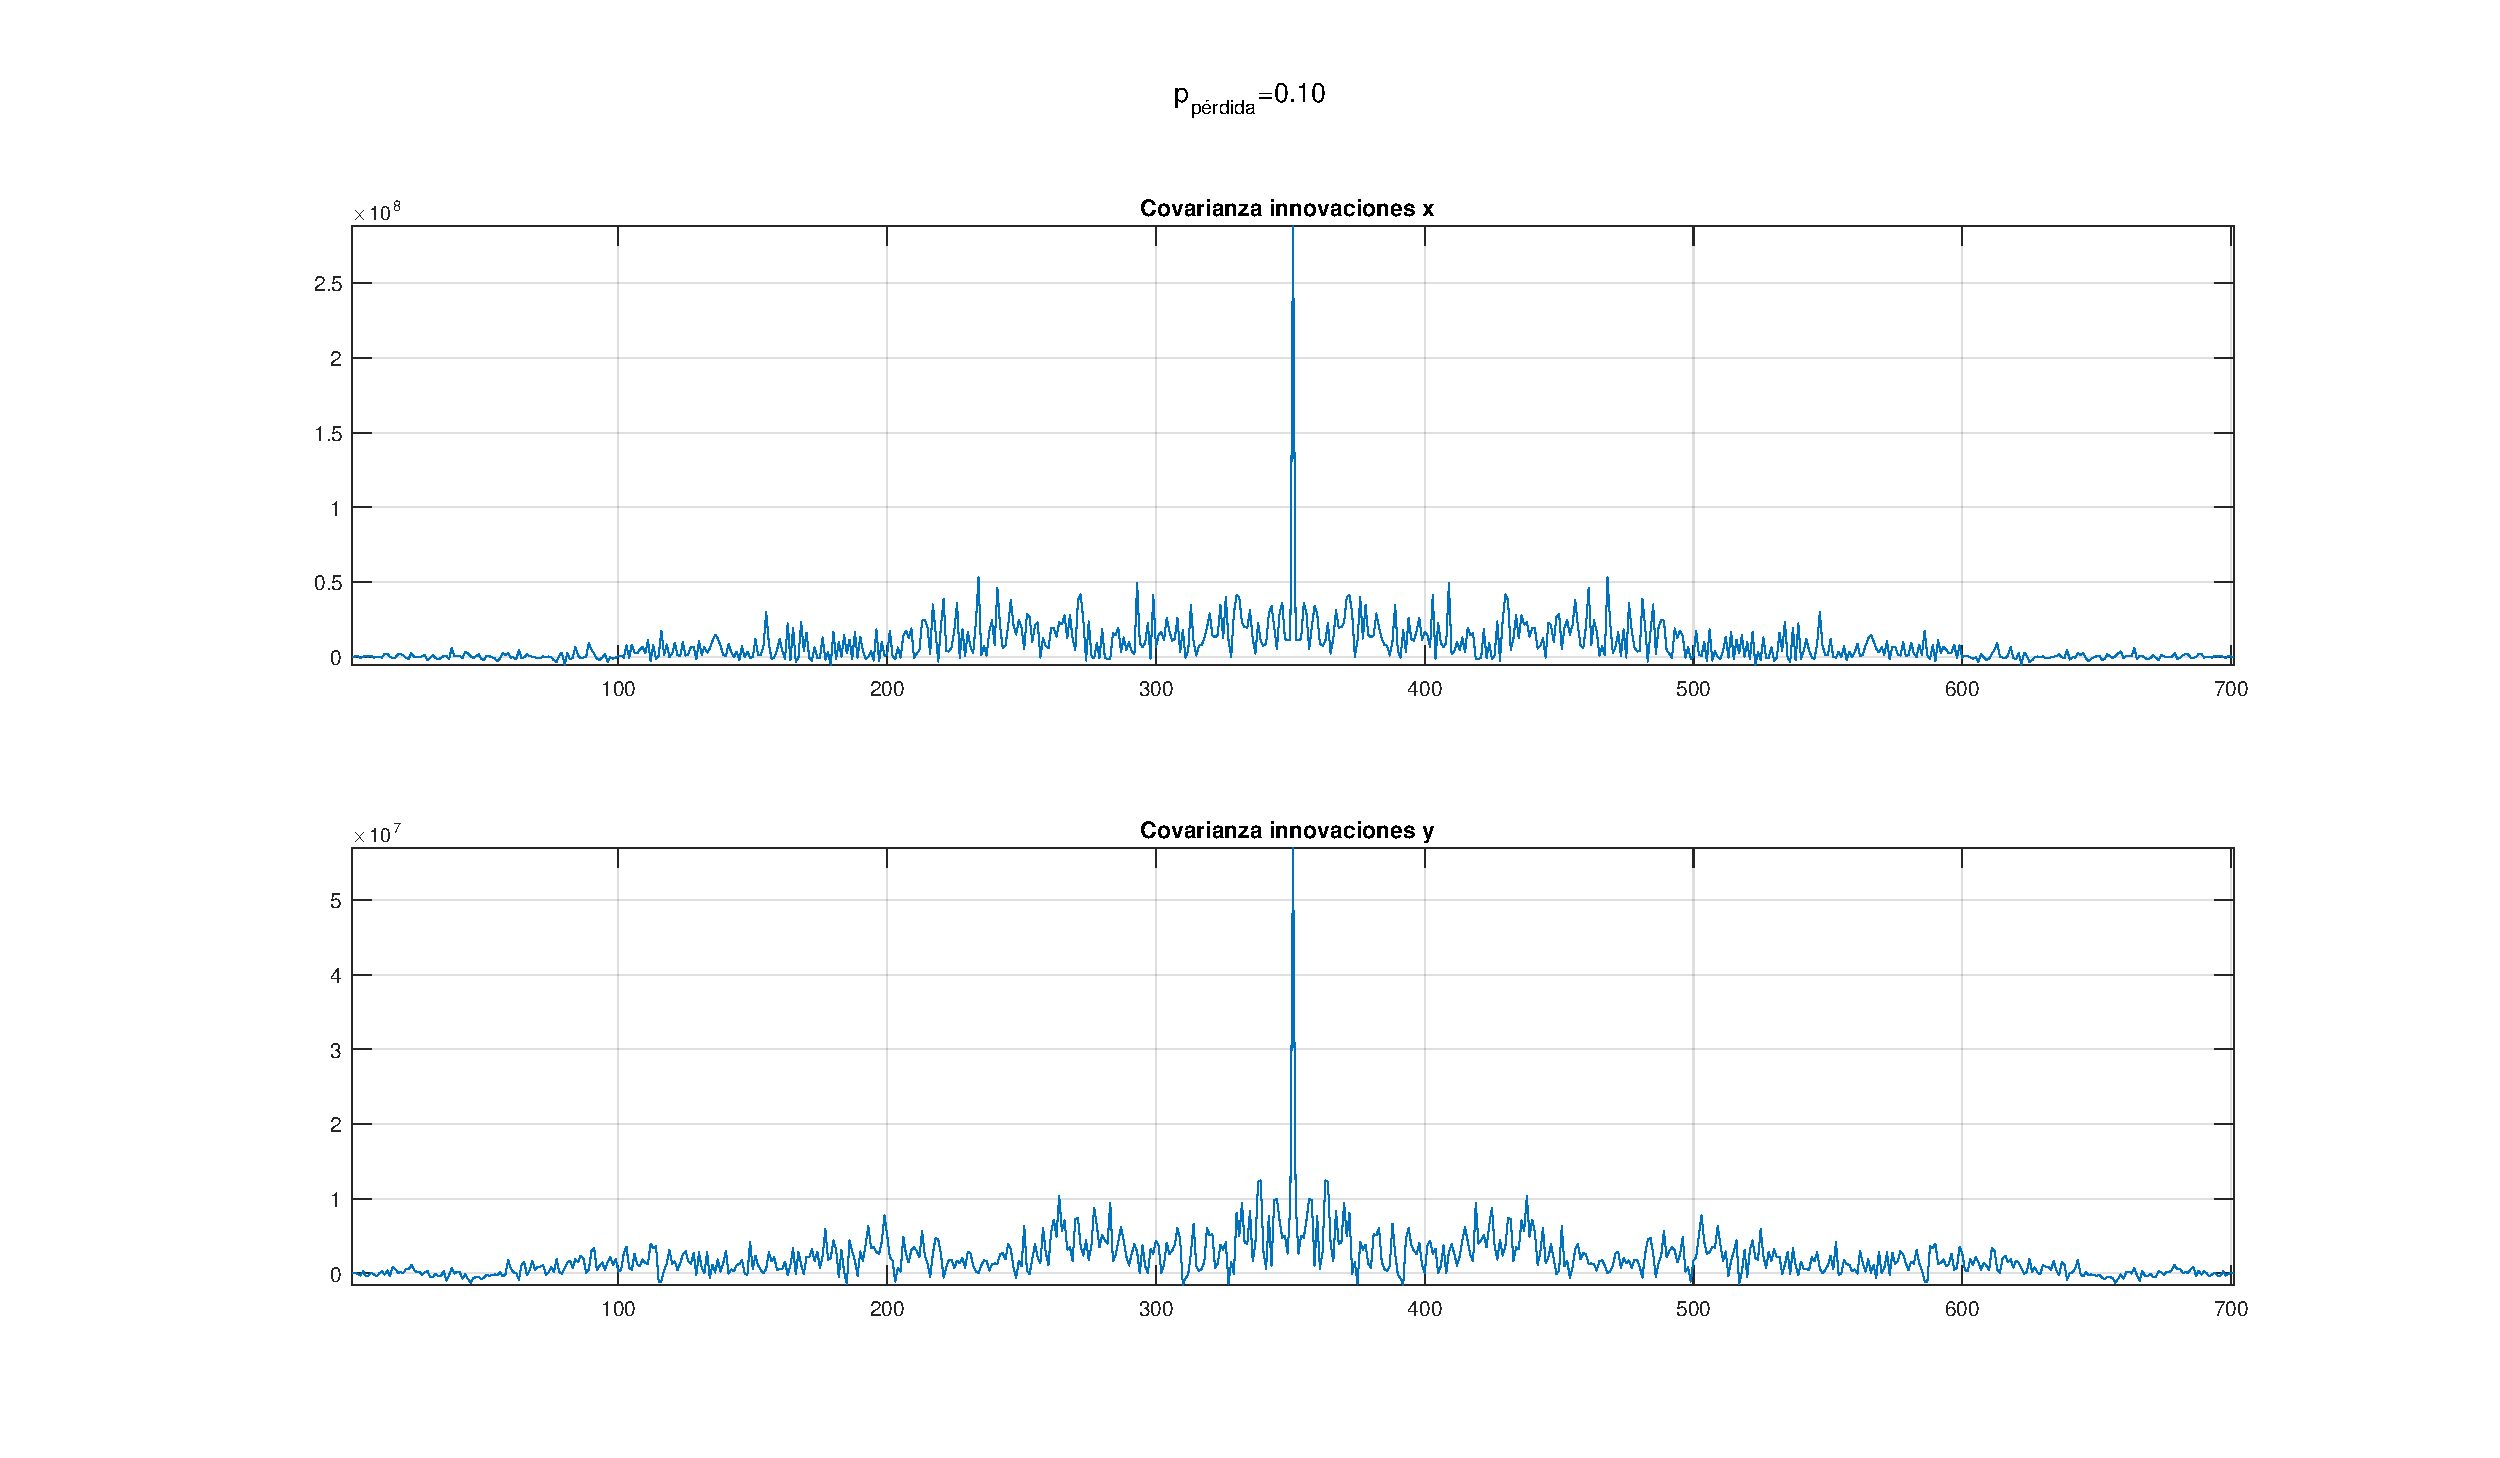
\includegraphics[width=1.0\textwidth,keepaspectratio]{Figuras/covinn_ej7_1.pdf}
		\caption{Autocorrelación De Innovaciones - Perdida Del 10 \%}
		\label{fig:ej7_1_inov}
	\end{figure}
	
	\begin{figure}[H]
		\centering
		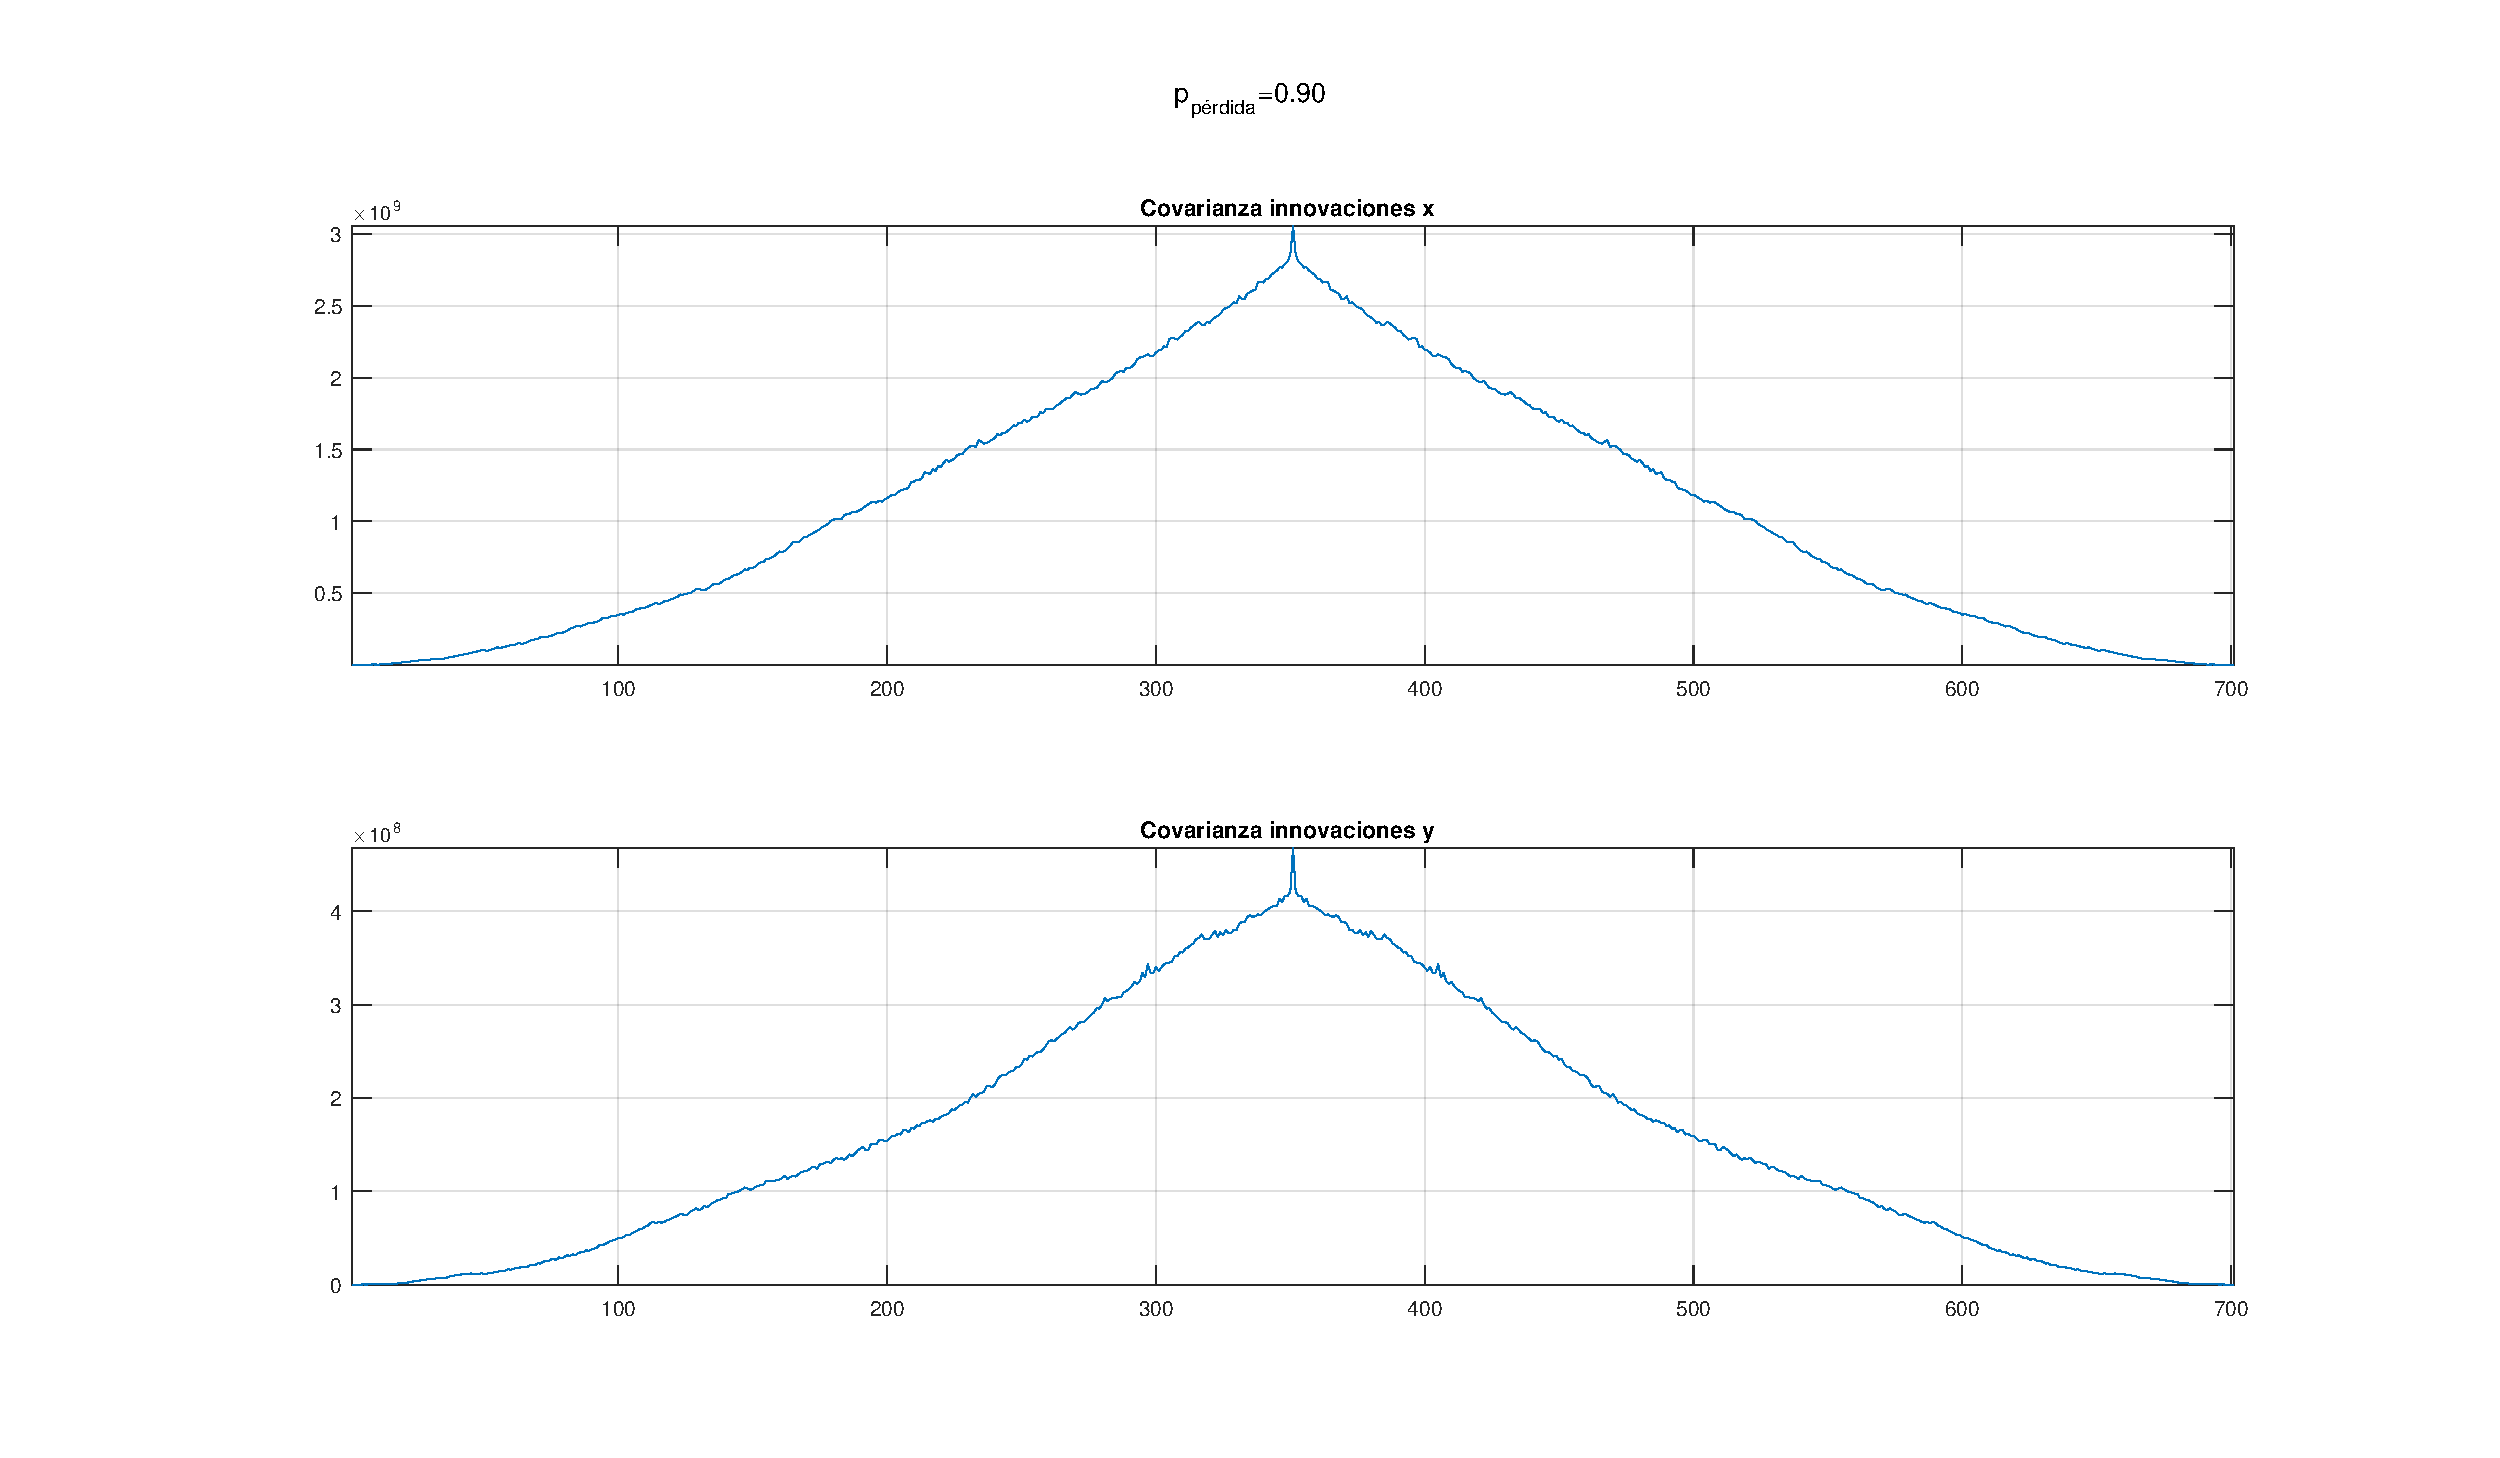
\includegraphics[width=1.0\textwidth,keepaspectratio]{Figuras/covinn_ej7_2.pdf}
		\caption{Autocorrelación De Innovaciones - Perdida Del 90 \%}
		\label{fig:ej7_1_inov}
	\end{figure}
	
	\subsection{Script}

	A continuación incluimos el script que realiza la estimación.
	
	%\lstinputlisting[]{../Octave/EJ7.m}
